\documentclass{standalone}
\usepackage{tikz}
\usetikzlibrary{shapes.geometric}
\newcommand\py{1.7}
\begin{document}
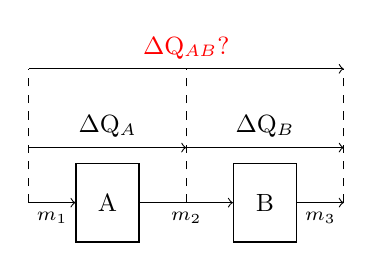
\begin{tikzpicture}[square/.style={regular polygon,regular polygon sides=4}]
    \node at (0, 0) [rectangle, minimum width = 0.8cm, minimum height = 1cm, draw] (o1) {\small A}; 

\node at (2, 0) [rectangle, draw, minimum width = 0.8cm, minimum height=1cm] (o2) {\small B};
    
    %DeltaQ marking above
    \draw [->] (-1, 0.7) -- (1,0.7) node[midway, above] {\small $\Delta$Q$_A$};
    \draw [->] (1, 0.7) -- (3,0.7) node[midway, above] {\small $\Delta$Q$_B$};
    

    \draw [dashed] (-1, 0) -- (-1, \py);
    \draw [dashed] (1, 0) -- (1, \py);
    \draw [dashed] (3, 0) -- (3, \py);
    
    \draw [->] (-1, \py) -- (3, \py) node[midway, above, red] {\small $\Delta$Q$_{AB}$?};
    %Relations events outcomes
    \draw [->] (o1.east) -- (o2.west) node[midway, below] {\scriptsize $m_2$};
    \draw [->] (-1, 0) -- (o1.west) node[midway, below] {\scriptsize $m_1$};
    \draw [->] (o2.east) -- (3, 0) node[midway, below] {\scriptsize $m_3$ };
\end{tikzpicture}
\end{document}

